\PassOptionsToPackage{top=3cm,left=3cm,right=3cm,bottom=3cm}{geometry}
\documentclass[fleqn,11pt]{wlscirep}

\usepackage{import}
\usepackage{main}

\renewcommand{\paragraph}[1]{\vspace{0.3cm}\noindent\underline{\emph{#1}}\hfill\noindent}

% word count
% \newcommand{\maincount}[1]{%
%   \immediate\write18{texcount -1 -sum=1 -merge -q -nobib #1.tex > #1-words.sum}%
%   \input{#1-words.sum}%
% }

% \newcommand{\abstractcount}[1]{%
%   \immediate\write18{texcount -template="{abst}" #1.tex > #1-words.sum}%
%   \input{#1-words.sum}%
% }

\begin{document}

\doublespacing

\title{\bfseries\LARGE\singlespacing{Spatiotemporal modeling of \emph{Mycobacterium tuberculosis} transmission risks using environmental, clinical, and patient movement data}}
% author list
\author[1$\ddag$]{Nicolas Banholzer}
\author[2]{Keren Middelkoop}
\author[2]{Juane Leukes}
\author[1]{Kathrin Zürcher}
\author[2]{Robin Wood}
\author[1]{Matthias Egger}
\author[1*]{Lukas Fenner}

\affil[1]{Institute of Social and Preventive Medicine, University of Bern, Bern, Switzerland}
\affil[2]{Desmond Tutu HIV Centre, Department of Medicine, University of Cape Town, Cape Town, South Africa}

\affil[*]{Corresponding author: lukas.fenner@unibe.ch }

\vspace{1em}

% \begin{information}\normalfont
% \noindent\textbf{Running head}: SARS-COV-2 transmission in schools and effect of air cleaners

% %\noindent\textbf{Subject categorization}: 6.20  Indoor Air; 10.11 Pediatrics: Respiratory Infections

% \noindent\textbf{Word count}: \maincount{manuscript}words, abstract \abstractcount{manuscript}words (max. 500), title 157 chars (max. 200)

% %\noindent\textbf{Inserts:} 2 tables, 6 figures, 44 references

% \noindent\textbf{S1 Appendix:} Includes supplementary text, tables and figures.

% \vspace{1em}

% \noindent\textbf{Funding}

% \noindent This study is funded by the Multidisciplinary Center for Infectious Diseases, University of Bern, Bern, Switzerland. NB, LF, and ME are supported by the National Institute of Allergy and Infectious Diseases (NIAID) through cooperative agreement 5U01-AI069924-05. ME is supported by special project funding from the Swiss National Science Foundation (grant 32FP30-189498). \medskip

% \noindent\textbf{Contributions}

% \noindent Conception and design: NB, LF. Epidemiological and environmental data collection: NB, PJ, TS, LF. Laboratory data collection: PB, LFu. Additional data collection: TH. Statistical analysis: NB, KZ. Genomic analysis: LB, LFu. Paper draft: NB, LF, ME. All authors reviewed and approved the final version of the manuscript.

% \par
% \end{information}

%TC:newcounter abst Words in abstract
%TC:envir abstract [] abst
\begin{abstract}\normalfont
\noindent\textbf{Background:} Tuberculosis (TB) caused by \emph{Mycobacterium tuberculosis (Mtb)} was the leading cause of death from any single infectious disease before the COVID-19 pandemic, and progress made before the pandemic has stalled or reversed. TB is mostly transmitted through the airborne route and the risk of transmission is thus higher in crowded indoor settings, especially healthcare facilities where both more infectious and susceptible people gather. Modeling the risk of airborne transmission is difficult and existing approaches, such as the Wells-Riley model, assume that the airspace is well-mixed, so that the spatial location of infectious and susceptible individuals is not considered.  \medskip

\noindent\textbf{Methods:} We develop a spatiotemporal model for estimating the risk of infection that builds upon the Wells-Riley model. We apply our model to environmental (CO$_2$ levels), clinical data (patient visits and TB status), and patient movement data (anonymized trackings from video sensors) that were collected for 5~days between October and November 2021 (during the COVID-19 pandemic) in a primary care clinic in Cape Town, South Africa. We link tracking and clinical data to identify the spatiotemporal location of TB infectious patients inside the clinic. Incorporating prior assumptions about the generation, diffusion, and removal of infectious doses (so-called quanta), we perform Monte Carlo simulation to estimate the personal risk of infection for each clinical attendee. We compare our simulation results with a non-spatial variant of our model and assess the correlation with characteristics of the clinical visit (\eg time spent in the clinic and the number of close contacts).
\medskip

\noindent\textbf{Results:} ...

\noindent\textbf{Conclusions:} ... 

\par
\end{abstract}

%TC:ignore

\flushbottom
\maketitle
\setcounter{page}{1}
\thispagestyle{fancy}

\vspace{2em}

%\noindent\textbf{Word count:} \abstractcount{manuscript}words (max. 500)

\vspace{0.5em}

\noindent\textbf{Keywords:} Mycobacterium tuberculosis, airborne transmission, spatiotemporal modeling, Wells-Riley model
% maximum of 3-5 keywords
\newpage

\sloppy
\raggedbottom
%TC:endignore

\newpage

%TC:break main
\section{Introduction} 

% TB and routes of transmission
Tuberculosis (TB) is one of the leading causes of death worldwide, especially in South-East Asian and African region\cite{WHO2022TBReport}. Progress made before the COVID-19 pandemic has stalled or reversed as the number of TB-related deaths have increased between 2019 and 2021 [TB report]. \emph{Mycobacterium tuberculosis (Mtb)}, the causative agent of TB, transmits via respiratory particles in the exhaled air of infectious person\cite{Rieder1999,Patterson2021Tuberculosis}. \emph{Mtb} is carried primarily in smaller particles $\leq5\mu$m called aerosols\cite{Fennelly2020Lancet}, which can survive in the air for multiple hours\cite{Loudon1969AMRRD}. Airborne transmission is more likely in crowded, poorly ventilated indoor settings\cite{Rieder1999,CPS2013Book,Nardell1991ARRD,Wang2021Science,Morawska2021}. Furthermore, there is a high risk of \emph{Mtb} infection in healthcare facilities, such as primary care clinics because both people that are more infectious and susceptible are also more frequently visiting the clinic\cite{McCreesh2020IJTLD}. A study in South Africa estimates that 4\% to 14\% of TB cases in adults originate from primary care clinics\cite{McCreesh2022BMJGlobalHealth}.

% the Wells-Riley model
The Wells-Riley model\cite{Riley1978AJE} is frequently used to estimate the risk of airborne transmission in a variety of indoor settings\cite{Andrews2014JID,Taylor2016IJTLD,Hella2017JInfect}, including primary care clinics\cite{Zurcher2022JID,McCreesh2021BMJGlobalHealth}. The Wells-Riley model assumes a well-mixed airspace, where the risk of infection is modeled as a function of the number of infectious individuals in space, the generation rate of infectious doses (so-called quanta), the breathing rate per person, and the outdoor air supply rate. The quanta generation rate (commonly denoted with the parameter $q$) is unknown, but can be estimated by computing the risk of infection as the ratio of diseased/susceptible cases, and then solving the Wells-Riley equation for the parameter $q$\cite{Nardell1991ARRD,Escombe2008PLoSMed}. The Wells-Riley model considers the importance of ventilation by which infectious quanta are removed from the indoor space through outdoor air exchange. While the ventilation rate is difficult to estimate, an alternative formulation of the Wells-Riley equation exists that uses indoor CO$_2$ levels as a marker of exhaled-breath exposure\cite{Rudnick2003IndoorAir}, which is related to the ventilation rate. 

% limitation of the Wells-Riley model
A crucial assumption of the Wells-Riley model is that the airspace is well-mixed, which means that there is no spatial variation in the exposure to infectious doses. Although it is reasonable to assume that infectious particles disperse in the indoor space over time, the aerosol concentration is at first highest closest to the infectious person\cite{Vuorinen2020SafSci,Chen2020BuildEnv}. Therefore, both short- and long-range transmission of \emph{Mtb} (and other pathogens) seem plausible. Nevertheless, previous studies show that the risk of infection is associated with proximity to an infectious person\cite{Ko2004RiskAnal,Kenyon1996NEJM}, which is in line with the hypothesis that prolonged close contact is required for transmission\cite{Leung2020NatMed,Brankston2007LancetID,Narasimhan2013PulmonaryMed}. However, proximity to an infectious person is not considered in the Wells-Riley model. It would also be difficult to test such a spatiotemporal extension of the Wells-Riley model because the location of the infectious and susceptible individuals are rarely observed.    

% what this study adds
We build on the Wells-Riley equation and develop a spatiotemporal model for the concentration of infectious quanta in the indoor space over time. We combine clinical and video tracking data to inform the spatiotemporal location of \emph{Mtb} infectious and susceptible individuals visiting a primary care clinic in South Africa between October and November 2021. Furthermore, we measure indoor CO$_2$ levels to model the diffusion and removal of infectious quanta over time. Our model allows us to identify spatiotemporal hotspots of quanta inside the clinic and estimate the risk of infection individually for each clinical attendee. We compare our modeling approach with an alternative specification that assumes a well-mixed airspace, thereby quantifying the contribution of close contact with infectious attendees to \emph{Mtb} transmission risk. 

\newpage

\section{Methods}

\subsection{Study design}

We build on the design of a pilot study in 2019\cite{Zurcher2022JID}, which was described in detail in a study protocol \cite{Zurcher2020BMJ}. In this follow-up study, we collected environmental data (indoor CO$_2$ levels), clinical (TB status), and tracking data (patient movements) on five days between October and November 2021 (October 13, 15, 25 and November 4, 5) at a primary care clinic in Cape Town, South Africa. Compared to the pilot study, we extended the patient tracking to include the TB treatment room. Molecular data was not part of the analysis of this study. 

\subsection{Study setting}

The primary care clinic offers both TB and HIV services and reproductive health and childhood immunization services, Monday to Friday, from 7\,am to 4\,pm. The clinic is situated within a large settlement of formal and semiformal housing where both TB and HIV are highly prevalent\cite{Wood2007AMJRCCD,Middelkoop2011JAIDS} [Wood 2007, Middelkoop 2011]. We delineated 3~areas within the clinic: the waiting room, the corridor, and the TB treatment room (Supplementary Figure~\zref{fig:floor-plan} in \supp). Furthermore, we defined two time periods: morning (7:00\,am to 12:00\,am) and afternoon (12:00\,am to 4:00\,pm). 

\subsection{Data}

\subsubsection{Environmental data}

Four devices monitored indoor CO$_2$ levels (Digital CO$_2$ Monitor Carbon Dioxide Meter XE-2000, XEAST, Guangdong, China) in the waiting room, corridor, and TB treatment room (Supplementary Figure 1). CO$_2$ concentrations were recorded in parts per million (ppm) at 1-minute intervals (Supplementary Table 1). Missing values were linearly imputed, except for October~13 where the corridor's CO$_2$ levels were almost completely missing. Here we assumed the same levels as in the waiting room because both rooms had also similar CO$_2$ levels on the other days.    

\subsubsection{Clinical data}

We extracted clinical data from the electronic patient registry for all patients who visited the clinic during the study period. These data included the date and time of arrival for the clinic visit, TB diagnostic results, and date of TB treatment start and (if applicable). We defined infectious patients as individuals testing positive for TB during the study or being on TB treatment since $\leq$28\,days. Patients who had completed a treatment were not considered infectious anymore.

\subsubsection{Tracking data}

We used an anonymized movement tracking system (Xovis, Zollikofen, Switzerland) to monitor people’s movements (staff members, patients, and other visitors) throughout the clinic (Supplementary Figure~\zref{fig:floor-plan} in \supp). The resulting date- and timestamped movement data consisted of a person’s height, their position recorded as x-y coordinates, and a unique ID for each person's track while in the clinic. Supplementary Figure \zref{fig:tracking-examples} in \supp shows a small, random sample of the tracks from our study. Note that individuals could contribute multiple tracks if they went out of a sensor’s range and subsequently returned or if they were briefly lost because the sensor did not recognize them as a person (\eg if bending or hiding behind another person). To link these tracks, we created a R Shiny tool and manually linked tracks back together that most likely belonged to the same person (Supplementary Text describing and illustrating the tool and automatic pre-matching). We defined close contacts as other persons passing within a radius of $\leq$1\,m. 


\subsection{Spatiotemporal modeling}

The workflow of our spatiotemporal modeling approach is shown in \Cref{fig:modeling-flow}. (1)~We combine patient tracking and clinical data to identify the spatiotemporal location of infectious individuals inside the clinic. We record the registration time for patients spending $\geq$5~seconds in the registration area, and then link their registration time with the nearest arrival time recorded in the clinical data, considering a maximum delay of 15~minutes. (2)~In addition to the number of TB patients masked from clinical data, we consider a similar number of unmasked TB patients among all other clinical attendees\cite{Berhanu2023CID}. Both masked and unmasked TB patients generate infectious quanta at their spatiotemporal location. The quanta generation rate $q$ is informed by estimates from the literature\cite{Andrews2014JID,Riley1962ARRD,Escombe2008PLoSMed,Nardell1991ARRD} and we apply a reduced rate to account for the effect of mask wearing\cite{Dharmadhikari2012AJRCCM}, which was mandatory in the clinic during the study period. (3)~We combine patient tracking and environmental data to monitor natural ventilation by computing the outdoor air exchange rate $AER$ from the number of people in the room and indoor CO$_2$ levels\cite{Batterman2017IJERPH}. (4)~The $AER$ is related to the diffusion constant $D$ (in m$^2$/s)\cite{Cheng2011EnvSciTech}, which determines the speed at which the infectious quanta spatially diffuses in the indoor air. We assume that the infectious quanta diffuses radially from the spot where it was generated. (5)~The $AER$ also corresponds to the rate of quanta removal through natural ventilation. The total removal further considers the viral inactivation rate $\lambda$, which is informed by prior literature\cite{Loudon1969AMRRD,Lever2000LettersAppliedMicrobio,Gannon2007ResVetSci,Klein2014IJMyco}. (6)~Quanta generation, diffusion, and removal determine the quanta concentration $N$ at time $t$ in the clinic, which is computed as 
\begin{align}\label{eq:spattemp-N}
    \underbrace{N_{t}}_{\text{new concn.}} = \underbrace{\left(D \Delta (\underbrace{N_{t-1}}_{\text{prev. concn.}} + \underbrace{I_t \cdot q}_{\text{generation}})\right)}_{\text{diffusion}} \cdot \underbrace{\exp\left(-(AER_t + \lambda)\right)}_{\text{removal}} ~.
\end{align}
where $\Delta$ is the Laplace operator (second-order differential operator) and $I_t$ is the number of infectious individuals in space. Finally, the patient-specific risk of infection depends on the cumulative exposure to infectious quanta during the clinical visit. We use the Wells-Riley Poisson relation to estimate the risk of TB transmission for each clinical attendee $a$ as 
\begin{align}
    P_a = \sum_s \sum_t N_{s,t} \cdot \mathbb{I}_{s,t}^a \cdot p,
\end{align}
where $P$ is the probability of infection, $\mathbb{I}$ is a binary variable indicating whether attendee $a$ was at location $s$ at time $t$, and $p = 8$\,l/min is the volumetric breathing rate per person. The general modeling framework together is described together with an example in detail in Text~\zref{sec:spattemp-model} in \supp. 

\begin{figure}[!htpb]
    \centering
    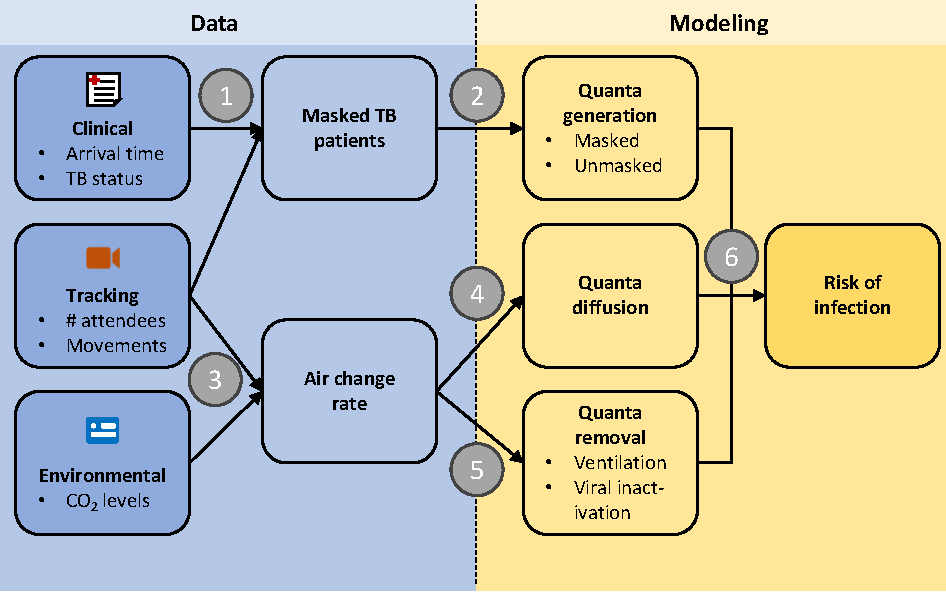
\includegraphics{doc/paper/flow-chart.pdf}
    \caption{Flow chart of the spatiotemporal modeling approach illustrating the steps from data (blue) to modeling (yellow).}
    \label{fig:modeling-flow}
\end{figure}

We divide each separate area of the clinic (waiting room, corridor, TB room) into a grid of cubic cells with an area of 0.25m$^2$ and a volume depending on the height of the room (waiting and TB room: 3m; corridor: 2.5m). We update the quanta concentration every second and assume that $N_{s,0} = 0 ~~ \forall s$, \ie all quanta from the previous day has been removed from the air before the start of the following clinical day. Due to mask wearing, we assume that the initial spread of quanta before diffusion is limited to the cell where the infectious individual is located. We model all model parameters with prior distributions and perform Monte-Carlo simulation to estimate the risk of infection. In each simulation, we perform the following three steps: (i)~sampling uncertain modeling parameters and undiagnosed TB patients, (ii)~computing the spatiotemporal quanta concentration, and (iii)~computing the cumulative risk of infection for each clinical attendee. The model setup, including the specific assumptions and prior distributions, is described in detail in Text~\zref{sec:estimation} in \supp.



\subsection{Statistical analysis}

We report the time-varying CO$_2$ levels, the daily number of registered and masked TB patients, and the number of clinical attendees monitored through patient tracking. We perform 10,000 Monte Carlo simulations and show the average quanta concentration by daytime and summarize the risk of infection with the mean and 95\%-credible interval (CrI) across simulations. To demonstrate the impact of spatial modeling, we compare our modeling approach with one that assumes a well-mixed airspace (\ie where the initial quanta concentration is the same everywhere in the room regardless of where it was generated). Furthermore, we assess the correlation between the personal risk of infection and characteristics of the clinical visit (time spent in each area, number and duration of close contacts). To assess the effectiveness of mask wearing, we compare our modeling results with a scenario where there is no reduction in the generated quanta and the initial spread is extended to the first-neighbouring cells of where the infectious individual is located. All analyses were performed in R software (version 4.3.1)\cite{RCoreTeam2023}.


\subsection{Ethics statment}

The University of Cape Town Faculty of Health Sciences Human Research Ethics Committee (HREC/REF: 228/2019); the City of Cape Town (Project ID: 8139), South Africa; and the Ethics Committee of the Canton of Bern (2019-02131), Switzerland, approved the study.

\newpage

\section{Results}

...


\FloatBarrier

\newpage

\section{Discussion}

% summary
We modeled the spatiotemporal concentration of infectious quanta, considering the location of infectious individuals (quanta generation), spatial dispersion (quanta diffusion), and natural ventilation (quanta removal). We found ... 


% critical appraisal of our results


% factors affecting quanta generation
The generation, dispersion, and survival of infectious particles in the air is subject to considerable uncertainty. Therefore, Wells\cite{Wells1955} introduced the concept of a ``quantum'' (infectious dose) to capture the stochastic nature of airborne transmission. A higher concentration of infectious quanta corresponds to a higher probability for an individual to get infected. The probability of infection is modeled with a Poisson relation and the Wells-Riley model considers multiple determinants for the generation and survival of infectious quanta. Nevertheless, transmission events are difficult to predict as the occurrence depends on multiple other factors that can broadly be categorized into (1)~environmental factors, (2)~properties of the specific pathogenic, and the (3)~infectiousness of infected and susceptibility of uninfected TB patients. 

(1)~Environmental factors are somewhat considered by our model using CO$_2$ as a tracer gas to estimate outdoor air supply. The combination of clinical and video sensor data further allows the spatial modeling of quanta generation. This makes our approach unique compared to existing modeling based on the Wells-Riley equation assuming a well-mixed airspace\cite{Riley1978AJE,Rudnick2003IndoorAir}. However, the radial diffusion of quanta assumed by our model may not reflect the actual airflow at the primary care clinic. The spatial dispersion of infectious particles is often simulated with computational fluid dynamics (CFD) models\cite{Vuorinen2020SafSci,Jung2021InfectChemo,Li2021BuildEnv}. CFD models can simulate a variety of diffusion patterns, which help researchers understanding the influence of airflow. For example, considering airflow can identify poorly ventilated indoor spaces where infectious particles circulate inside the room rather than getting replaced with fresh air\cite{Li2021BuildEnv}. However, airflow is rarely considered and it may be difficult to assess in a naturally ventilated space, such as our primary care clinic, where it depends on the outdoor wind direction and which doors and windows are open. 

(2)~Survival and dispersion of aerosols are also determined by the physicochemical properties of virus-laden aerosols such as particle size, viral load, and other chemical components\cite{Wang2021Science}. Currently, these properties are only indirectly incorporated in our model by modeling the quanta generation rate as a stochastic parameter. It is also challenging to consider these properties because environmental factors, in particular temperature and humidity, can affect particle generation and survival, but the effects are often unclear and depending on the pathogen\cite{Songer1967,Chan2011AdvVir,Fernstrom2013JoP,Cox1995Book,Fernstrom2013JoP,Tang2009Interface}. Survival of bacteria in aerosols decreases with temperatures $>$24$^{\circ}$C, but the effects of humidity are unclear\cite{Tang2009Interface}. On the one hand, a comparison between two studies suggested that a higher survival rate of airborne \emph{Mtb} may be attributed to lower relative humidity\cite{Loudon1969AMRRD,Lever2000LettersAppliedMicrobio}. On the other hand, airborne \emph{Mtb} was more likely to be detected in healthcare facilitates with larger relative humidity\cite{Sornboot2019IJTLD,Matuka2021IJERP}.   


(3)~Previous studies show considerable variation in the generation of infectious quanta by TB infected patients\cite{Escombe2008PLoSMed,Andrews2014JID}. We model such variation by using a wide prior distribution for the quanta generation rate. Our model could be easily extended to incorporate prior information on the infectiousness of each individual TB patient. In general, only patients with active pulmonary TB are able to produce infectious droplets\cite{Rieder1999}. Infectiousness could be determined based on the most recent sputum test result. Sputum smear positive patients are more likely to transmit \emph{Mtb} than sputum smear negative patients\cite{Shaw1954ART,Brindle1993AMRRD,Grzybowski1975BIUT}. HIV status could further inform both infectiousness and susceptibility. On one hand, HIV-positive patients are more likely to have a negative sputum smear microscopy result than HIV-negative patients, due to the reduced lung cavitation and the fewer \emph{Mtb} bacilli in their sputum\cite{Brindle1993AMRRD,Telzak1997CID}. On the other hand, HIV-positive patients are less prone to control the \emph{Mtb} infection than HIV-negative patients, due to their reduced immune status\cite{Forte1992AIDS,Kwan2011CMR,Shen1988CEI}, and therefore TB disease progresses faster and is often more severe in HIV-positive TB patients compared to HIV-negative patients. 

% data and other limitations
While we combined multiple data sources to allow spatiotemporal modeling of the generation, spread, and removal of infectious quanta, our data has also limitations. First, clinical attendees could not always be tracked perfectly throughout the clinic using our video sensors. We invested considerable effort to manually link individual tracking IDs probably belonging to the same attendee back together (see Appendix), but some measurement error remains. Second, we linked video tracking and clinical patient data using the times clinical attendees were at the registration and the entry times in the clinical database. False linkages could result when a tracking ID only passed by the registration (without registering) or when multiple IDs were at the registration closely before a clinical entry. Third, to facilitate modeling, we considered the waiting room and corridor as separate, although the door between both rooms was usually open (\zref{prep:building} in \supp). Fifth, our video sensors could not cover the whole area of the entrance and we did not collect data in the care rooms and other places of the clinic. As a result, the time spent in the clinic and the exposure to infectious quanta may be underestimated for some clinical attendees, although we expect the largest exposure to be in the waiting room, which was fully covered.   

% conclusions
We conclude ...


\newpage


%TC:ignore
\section*{Acknowledgements}
...

\bibliography{references.bib}
%TC:endignore

\end{document}
